\chapter{Conceptual Model}\label{chap:conceptual_model}

The Conceptual Model section describes the research focusing on power optimization in Thread mesh wireless networks as part of the MOOD-Sense initiative. The primary goal is to improve energy efficiency in IoT applications utilizing the Thread protocol. The project will investigate and evaluate power optimization techniques and their impact on the overall network performance, contributing to the development of energy-efficient IoT networks.

The system will be developed based on the Thread protocol, a low-power, IPv6-based networking protocol designed for IoT applications. To optimize the power consumption of Thread networks, the project will employ a two-step process. First, the Monte Carlo Method will be used to find the optimal network configuration and initial transmission power. This step will involve a thorough analysis of different network configurations based on different constraints. The project will leverage MCM's strengths in randomness and theoretical justification to ensure the reliability of the results. Next, the Genetic Algorithm will take the final output from MCM and focus on finding the lowest transmission power possible. The use of GA will help improve the overall energy efficiency and performance of the Thread network by taking into account the network's constraints. The following diagram illustrates the flow of the entire process, from MCM and GA optimization to the implementation of optimized transmission power in the Thread network that shows a clear visual representation of the project's methodology.

\begin{figure}[H]
    \centering
    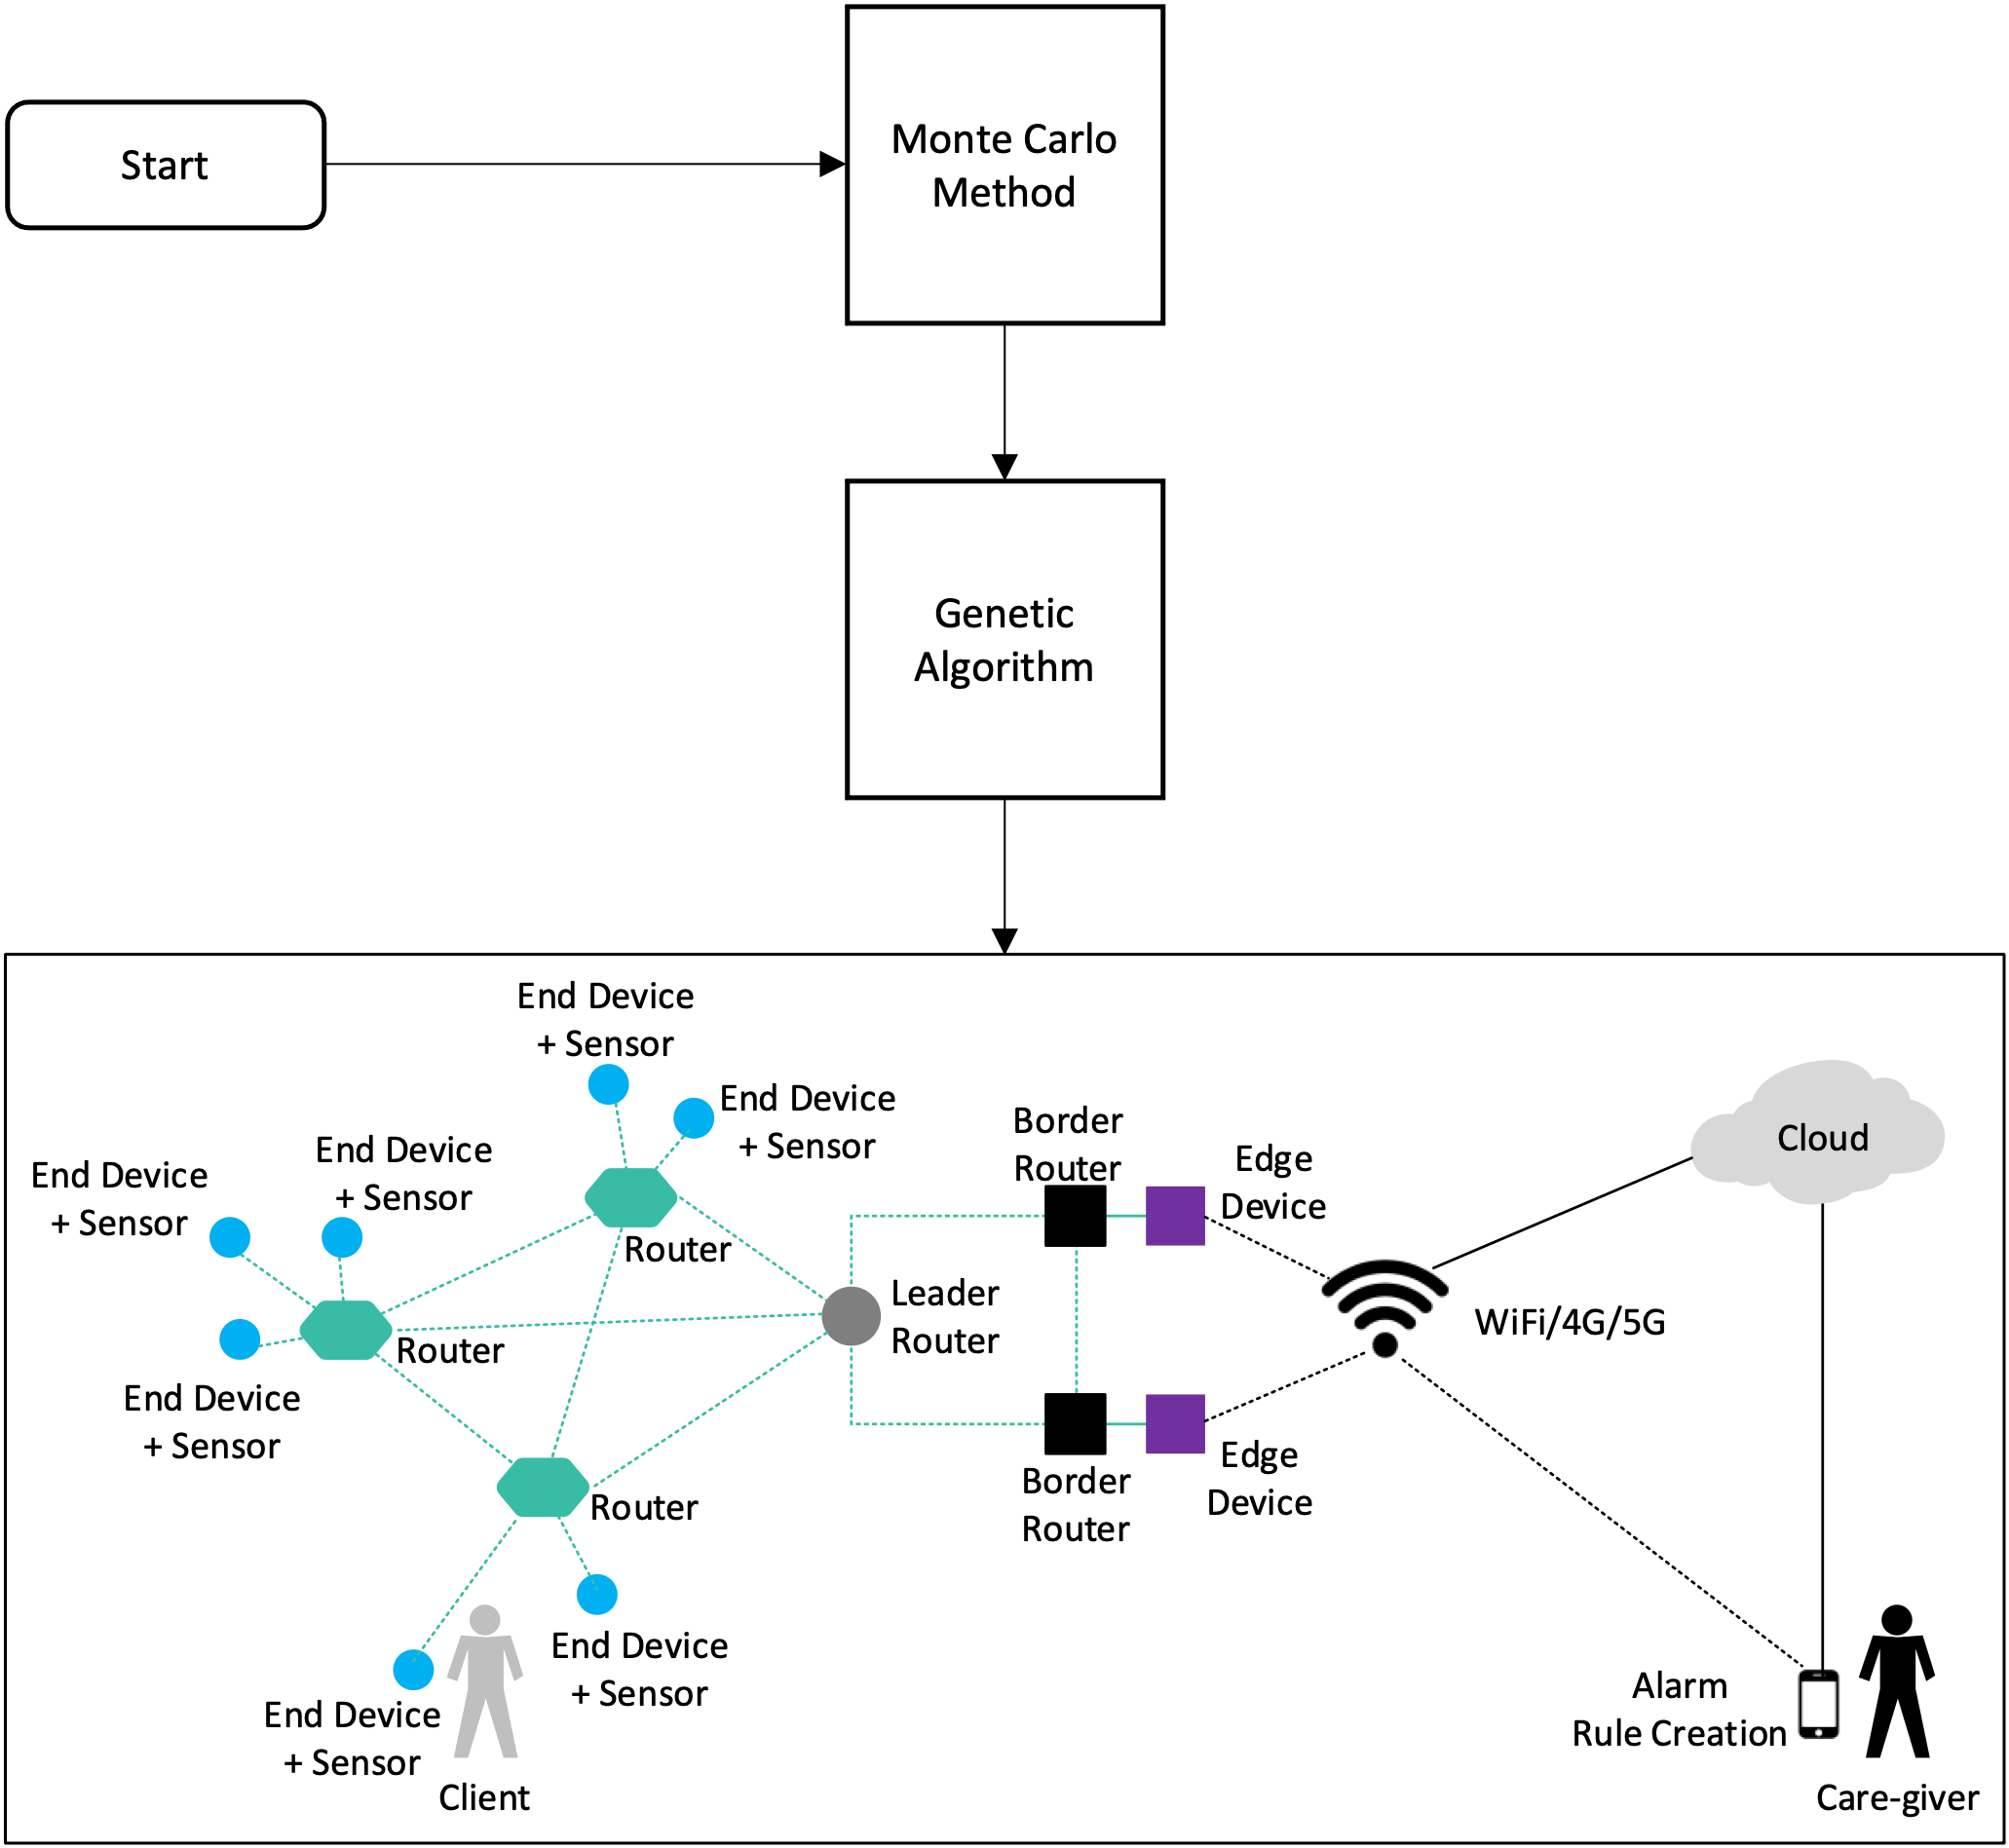
\includegraphics[width=0.8\textwidth]{images/conceptual_model/Thread_Network_Power_Optimization_Conceptual_Model.png}
    \caption{Thread network power optimization conceptual model.}
    \label{fig:conceptual_model}
\end{figure}

The project will consider the cost of hardware components, software development, testing, and deployment while maintaining a balance between cost-effectiveness and performance. The power consumption will be measured using Power Profiler Kit II explained in hardware section. The research will measure output power in different scenarios to validate the effectiveness of the power optimization techniques employed. These scenarios will be categorized based on the method, location, type, mode, duration, and ping used for power optimization and measurement.

\begin{enumerate}
  \item \textbf{Method}: The power consumption will be measured in two primary scenarios - Maximum and Optimized. The Maximum scenario represents the baseline power consumption, where no optimization techniques are applied. The Optimized scenario will measure power consumption after implementing the MCM and GA optimization techniques.
  \item \textbf{Location}: The measurements will be conducted in two different locations - Lab and Home. The Lab setting is smaller in size compared to the Home location, allowing for controlled environments and reproducible results. The Home setting provides a real-world context, with a larger area, helping to understand the performance of the Thread network in everyday IoT applications.
  \item \textbf{Type}: The power consumption measurements will also be conducted based on the type of network activity. The No Sensor scenario represents a Thread network with no active sensors, while the Ping scenario simulates data exchange between nodes, resembling real IoT network behavior.
  \item \textbf{Mode}: The project will compare the effectiveness of MCM and GA optimization techniques. The MCM mode will measure power consumption based on network configurations optimized using the Monte Carlo Method. The GA mode will measure power consumption with network configurations optimized using the Genetic Algorithm.
  \item \textbf{Duration}: The power consumption measurements will be conducted for different durations - 60 seconds in the Lab location and 300 seconds in the Home location. This variation in duration will help in understanding the impact of time on power consumption in different environments.
  \item \textbf{Ping}: In the Lab location, 50 pings will be sent within the 60-second duration, whereas in the Home location, 290 pings will be sent during the 300-second duration. This distinction will help analyze the impact of network activity on power consumption in both controlled and real-world settings.
\end{enumerate}

By measuring power consumption in these different scenarios, the research will provide a comprehensive understanding of the power optimization techniques' effectiveness. The results will be analyzed to draw comparisons and determine the optimal approach for power consumption reduction in Thread networks, ultimately contributing to the development of energy-efficient IoT networks.

In terms of sustainability, the research will emphasize energy-efficient hardware and power optimization techniques to minimize environmental impact, leading to sustainable IoT network deployments. By focusing on energy efficiency, the project inherently follows sustainable work principles, addressing resource conservation and minimizing negative impacts on society and the environment. Moreover, the research process involves the application and development of professional skills, such as data analysis, algorithm design, and critical thinking, to ensure the reliability and relevance of the results.

By combining the use of MCM and GA to optimize power consumption in Thread networks and employing sustainable work principles, this project will contribute valuable insights to the field of energy-efficient IoT network design and implementation.
